% This Source Code Form is subject to the terms of the Mozilla Public
% License, v. 2.0. If a copy of the MPL was not distributed with this
% file, You can obtain one at http://mozilla.org/MPL/2.0/.

\documentclass[11pt]{article}
\usepackage[utf8]{inputenc}
\usepackage{geometry}
\usepackage{graphicx} 
\geometry{a4paper} 
\usepackage{listings} % necessario per inclusione codice sorgente
\usepackage{color} % syntax highlighting
\usepackage{url}

\usepackage{amsmath}
\newcommand\ceil[1]{\lceil#1\rceil}
\usepackage{amsfonts}
\usepackage{amssymb}
\usepackage{pdfpages}
\usepackage{enumitem}

\pdfinfo{
   /Author (Marco De Nicolo)
   /Title  (Manuale Utente di Lost in Space)
}
\title{Manuale Utente Progetto Basi di Dati\\Lost in Space}

\author{Marco De Nicolo\\ matricola: 871524\\ \url{marco.denicolo@studenti.unimi.it}}

\date{Gennaio 2018}

\begin{document}
\maketitle
\newpage
\section{Installazione dell'applicazione}
L'installazione dell'applicazione richiede:
\begin{itemize}
\item apache 2.4+
\item python 3.4+
\item PostgreSQL 10+
\item PL/Python 3+
\item PHP 7+
\end{itemize}
\section{Configurazione della Base di Dati}
Per creare e popolare la base di dati servirà il file LiS\_dump.sql.
Il proprietario della base di dati è \textit {utente}, per cambiarlo bisogna modificare il file Lis\_dump.sql sostituendolo con il nome del proprio user.\\
L'utente deve essere superuser per poter utilizzare PL/Python come linguaggio procedurale.
\subsection{Esempio di configurazione con Postgresql per Linux}
Bisogna creare una base di dati chiamata LiS e scrivere in un terminale, aperto nella cartella del file dump, i seguenti comandi:\\
\$ createuser -s utente\\
\$ createdb -O utente LiS\\
\$ psql -d LiS -U utente -W \textless  LiS\_dump.sql\\
\section{Giocare a Lost in Space}
\subsection{Registrazione e Login}
Ci si registra inserendo nome, e-mail e password.\\
Per il login bisogna inserire nome o e-mail e la password.\\
\newline
\begin{center}
\fbox{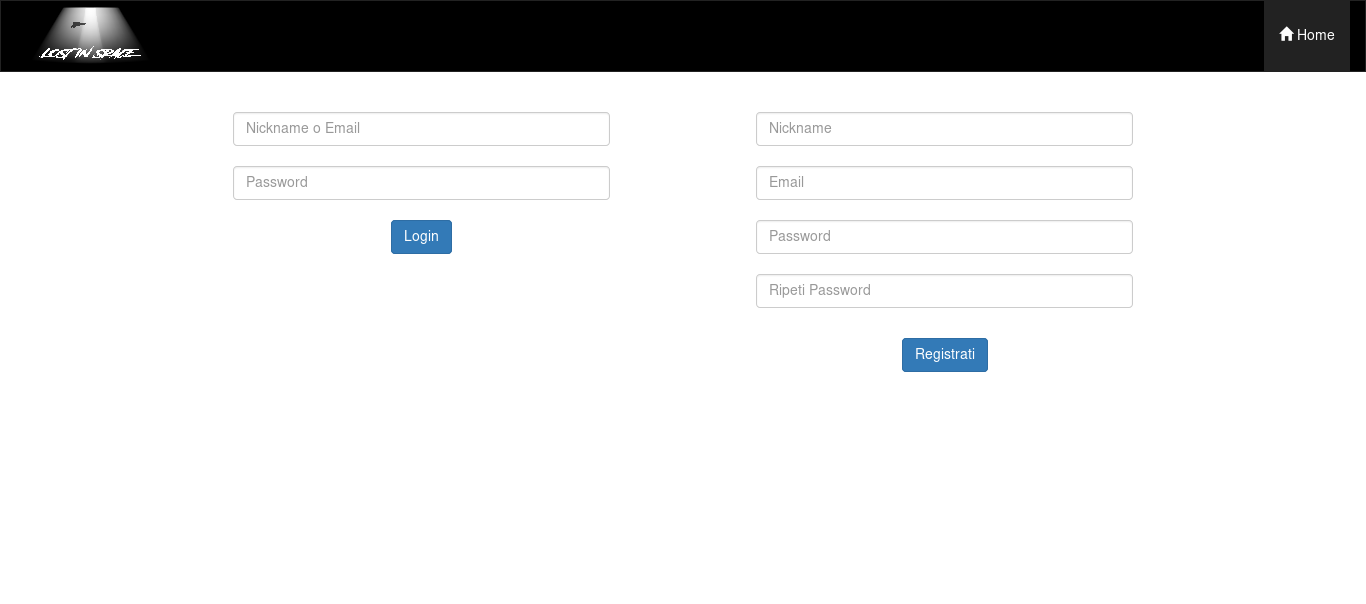
\includegraphics[scale=0.3]{immagini/reglog.png}}
\end{center}
\subsection{Gestione del Personaggio}
Per creare un nuovo personaggio è sufficiente inserire un nome, la descrizione è facoltativa.\\
Premendo "Inizia Avventura" si entrerà all'interno del Dungeon.\\
Con il tasto "X" verrà eliminato il personaggio.\\
\newline
\begin{center}
\fbox{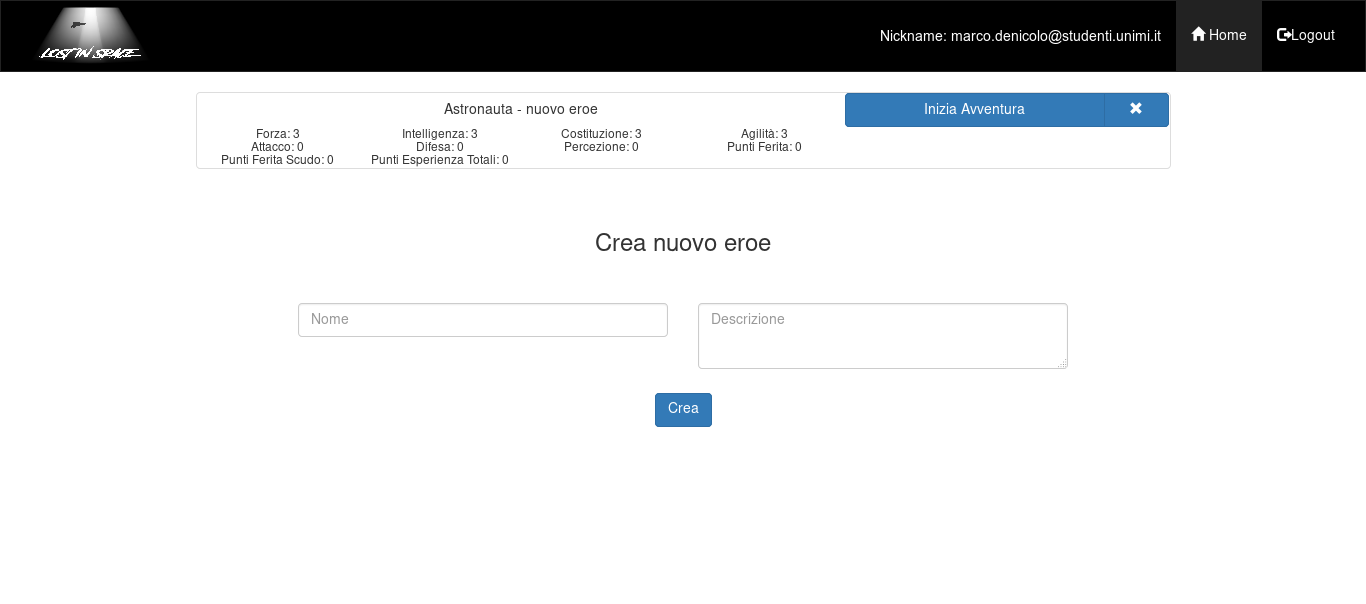
\includegraphics[scale=0.3]{immagini/creainizia.png}}
\end{center}
\subsection{Selezione dei Dadi}
Prima di iniziare un'avventura bisognerà scegliere quattro dei cinque valori, casuali, da assegnare alle rispettive abilità.\\
\newline
\begin{center}
\fbox{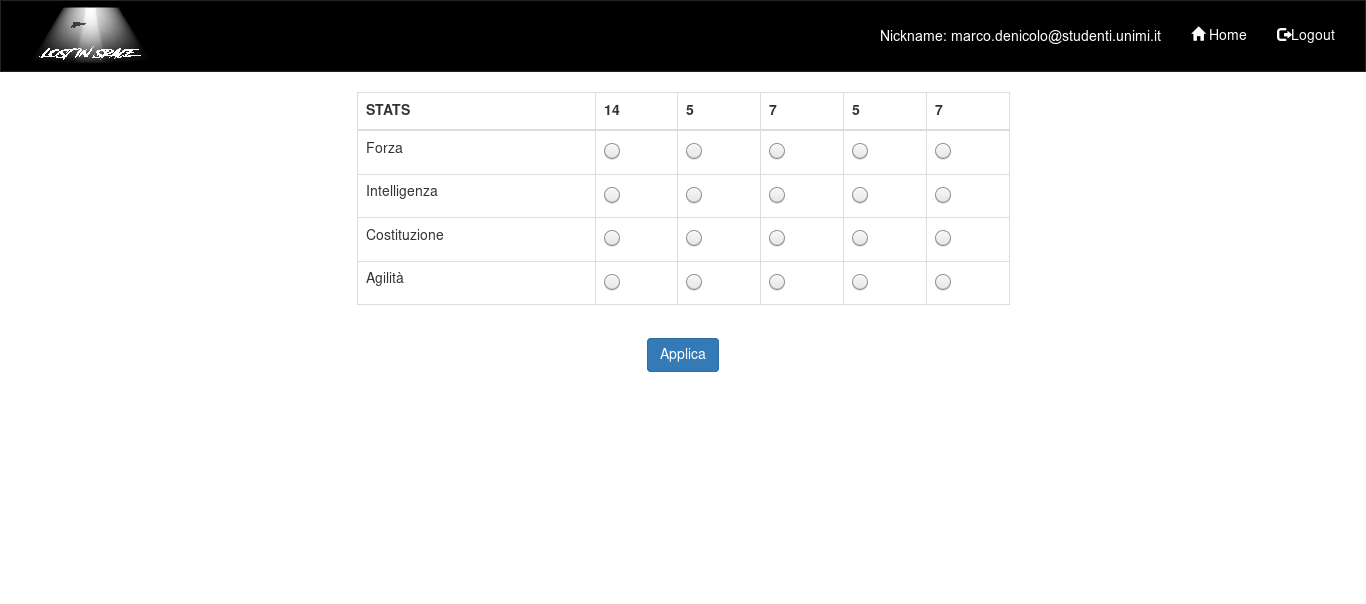
\includegraphics[scale=0.3]{immagini/dadi.png}}
\end{center}
\subsection{Schermata di Gioco}
Nella schermata di gioco ci sono tutte le informazioni riguardanti la stanza, i nemici, gli oggetti che possono essere raccolti, i collegamenti a stanze adiacenti, le statistiche e lo zaino del personaggio.\\
Gli oggetti equipaggiati hanno uno sfondo verde.\\
Il colore del contorno di un oggetto indica la sua tipologia:
\begin{itemize}
\item rosso: oggetto d'attacco
\item blu: oggetto di difesa
\item grigio: oggetto consumabile e valido per tutta la durata del gioco
\item arancione: oggetto consumabile e valido in una stanza sola, aumenta lo scudo e non i PV
\end{itemize}

Appena entrati in una stanza si viene attaccati dai nemici, bisogna quindi assicurarsi di avere abbastanza PV.
Durante un attacco i danni verranno sottratti dallo scudo e poi dai PV.
\begin{center}
\fbox{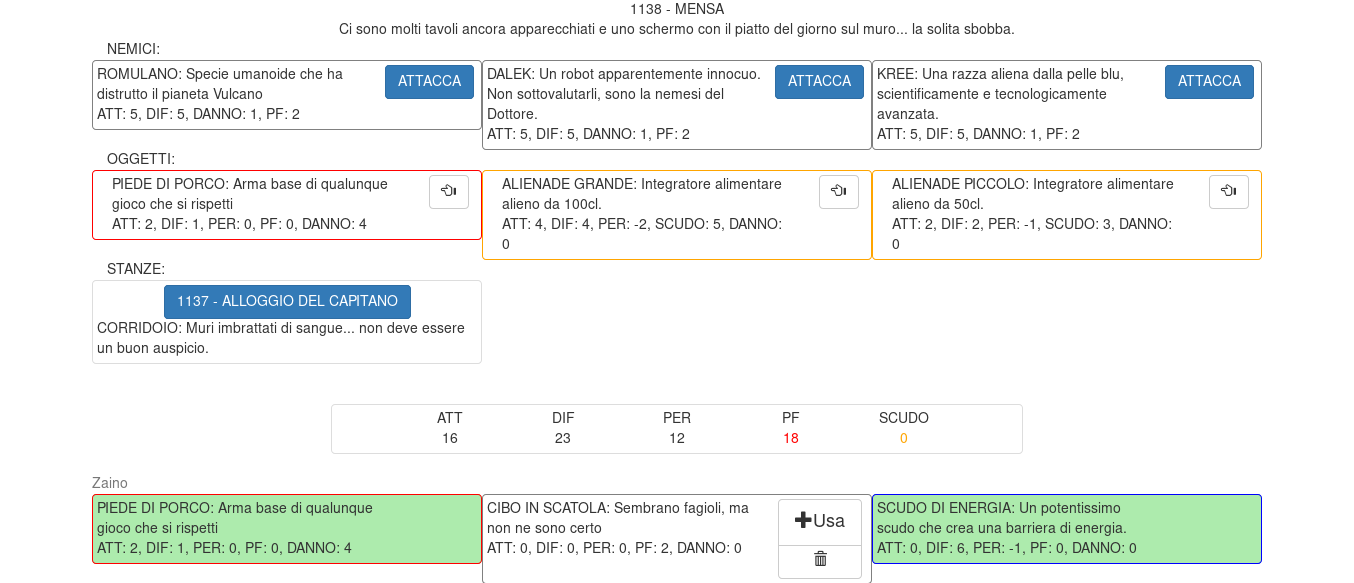
\includegraphics[scale=0.3]{immagini/gioco.png}}
\end{center}
 
Una volta eliminati tutti i nemici si potrà tentare la sorte, cercando degli oggetti o collegamenti nascosti all'interno della stanza, al costo di 1 PV.
\begin{center}
\fbox{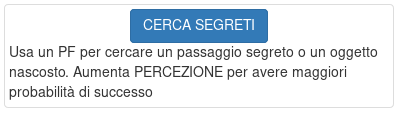
\includegraphics[scale=0.6]{immagini/cerca.png}}
\end{center}

\subsection{Fine dell'Avventura}
Se i PF scendono a 0 la partita termina e si viene riportati nella pagina di selezione del personaggio.\\
Quando si entra nella stanza finale la partita si conclude con la scritta "HAI VINTO!" ed un aumento dei punti esperienza.\\

\end{document}
